% Chapter 1
\setstretch{1}
\chapter{Introduction: A Better Time-Based Installation}\thispagestyle{empty} % Main chapter title

\label{Chapter1} % For referencing the chapter elsewhere, use \ref{Chapter1} 

\lhead{Chapter 1. \emph{A Better Time-Based Installation}} % This is for the header on each page - perhaps a shortened title
\setstretch{2}
%----------------------------------------------------------------------------------------
%	Abstract
%----------------------------------------------------------------------------------------
\section{Introduction}
What constitutes good design? As described by Don Norman in the book "The Design of Everyday Things," \parencite{norman} design can be sympathetic to their users, or have psychopathy coded directly into the construction of design artefacts. In response to this, I have designed a web application called screenPerfect to display synchronous multi-video screens and branched video narratives, and then a hardware solution that relies on the Raspberry Pi hardware architecture for installation. 

ScreenPerfect is distinct from pre-existing engines, written to encourage video artists to use their own skillset to explore what is possible in an interactive experience. ScreenPerfect's game-side interaction mechanics emphasize a classic branched narrative structure similar to that of FMV games, which can then be extended by any programmer to encompass new features. The editing and interaction mechanic are both straightforward to use and not designed to be altered by artists. This means that artists have a consistent environment in which to place their work, which will reliably showcase that work without them needing to learn how to program - an entirely new creative skillset – in order to do so.

This project has several parts which will be explained separately. The first part of the project is an application to build branched narratives out of video files, coded in javascript on the Node.JS framework for distribution via common internet technologies. This portion of the research has to do with the idea of structural political resistance through technology - implicit control systems - and how human abilities can be expanded by using contemporary technology, which is made by trained technicians but then released to be used without a proscriptive definition of the final use case. Although the intention is to make games, the software does not prevent, and even encourages, other uses. Users make use of the engine, developed through one specific user's design practice, to design new things. The first section of this paper presents how such an engine might be applied to video works.

The second part of this paper addresses how to perform user testing via a game jam format, a type of design charette in which users are given access to tools and asked to produce art with them. In that section, I document how No Jam 2: VideoVideo worked, the industry paired advantages to new engine development, and how this expands community ties for local artists working in a medium that frequently demands more collaboration than traditional, less dynamic art works.

In the third part of this paper, I address the issue of new media art and display. New media, particularly time-based media, is very challenging to display and support. Even low-end computers are bulky and expensive to deploy, so I have asked how we might circumvent traditional white-cube galleries while restricted by the requirements of internet technologies. In this part I detail how to build a server on the raspberry pi platform, a microcomputer, to deploy web-based applications to localized, internet-restricted spaces.
In conclusion, I argue that we need technology to belong to its users, instead of pursuing an exclusive reliance on mass network technologies. I feel that there has always been room for the technical in art, and while good technology fades into the background to leave only the artwork on display, the technology we choose to use provides the frame of what can be pursued.

\section{Designing Software to Power Experience}
The arts and the humanities are the technical name for the fields of work that produce both culture and its record of its culture. We use computers to do most white-collar office work. Machines automate and extend our ability to speak in repeatable patterns \parencite{glanville}. Repetition is a key component of mass production. Looked at as a tool, a computer is not so much a hammer as it is an ongoing negotiation - the user must decide what the black box means \parencite{glanville}.

The use of computers as tools requires a specific skill set that is as unique as the skill set of using a paintbrush. A key aspect of computer skill is a comfort with curiosity: digital tools change all the time, and many of them are not well written. Software is frequently unreliable, and hardware more so. Almost all software tools require time invested in skill acquisition before content - art - can be produced, and this time is expensive. The construction of the tools is an art, because when manufacturing a tool, it needs to be easily used, but it also needs to do something in a predictable, reliable way. A good digital tool should encourage rather than impede expression.

Artists, as a rule, have their own working methods and vision for their work in advance of picking up any new tool. For the purposes of this work, it is assumed that users have their own vision independent of the tool itself, which can be expressed, expanded, or extended by the use of a new tool. Ideally a tool vanishes in its use. It is a multiplier of force, where force can also be construed as capital, which could be the capital of knowledge and cultural membership, an availability of time to develop knowledge and then use the knowledge to operate in a space, or a more conventional type of currency: money.
Television and video are a format traditionally requiring capital to access. Culturally, video works - film and television - express mass ideals to mass audiences. YouTube, Vimeo, and visual FX production continue to drive technological innovation in systems development. Here I conflate instant film produced on a mobile phone with years of work in film production because the internet has flattened the effort it takes to consume media, if not its production. Most large-budget films in 2014 movies have at least some visual effects post-production. Some, such as "Life of Pi," are almost entirely composed of vFX and compositing, practice that requires years of skilled labour \parencite{lifeofpi}. Acquiring editing and image-design skills to work with moving pictures is an expensive and time-consuming pursuit, but putting any video at all on the internet takes almost no effort in centers with access to broadband internet. The advent of Vine and YouTube has democratized video to the point where it can be traded as words once were – or pirated, as the popular works of Dickens commonly were in early America \parencite{dickenscastillo}. Streaming media sites present an awkward effort to access larger works, but not by much, and Netflix's distribution model means that a year of filming work – in the case of House of Cards \parencite{houseofcards}, more than twenty hours of original television – has been redesigned to be consumed at the convenience of the audience. Spoilers now encourage watching the series inside a week, rather than over a month, or a year.

This moves the value of a given video experience from the control of the video producer to the audience. Rather than being restricted in a viewing experience to a theatre, the audience now decides where and how to consume popular works. Video is consumable on every kind of screen, especially on the smartphone screen. This permits acquisition of a broad audience, even as it shifts the context of the work.

A single smartphone in 2014 is more than powerful enough to supply most of the serving needs of previous video works, including branched narratives that once required many VCRs and multiple screens. As things become more accessible, according to Walter Benjamin \parencite{benjamin} they lose their aura, their singular magic, which means that accessing that magic becomes more challenging as the distribution of the work becomes easier. Partly, this seems to be a process of decontextualization: no matter how good a given film, it may be better in a theatre, en masse, because the theatre, its particular context, makes the experience of the film singular, even as the film itself is limitlessly reproducible.

The question in this context becomes: how to best retain the monetary and chronological capital of artistic tool use, vision, and creative practice, while restoring the aura of presentation required to engage with art on its own terms? How to expand artistic tool use into new means of expression? How to make use of contemporary methods in a way that may remain accessible and on display for years to come?
 
\section{Interaction and Presentation in Game Design}
In the context of this paper, my frame for the term "art" is digital games as interactive experience. In this case, technology design and game design must be considered together, in that the design of an experience is dependent on its technology.

That games are art, or can be art, has been popularly contested. Famously, in 2005, Roger Ebert took the position that games could never be art \parencite{ebert1}. He recanted this statement in 2010, with a public admission of bullheadedness and a confession that he simply did not wish to engage with games as a form \parencite{ebert2}. The debate has been reasonably settled, to my mind, with the rise of conferences such as Different Games NYC and Indiecade, with experiences at all investment levels to explore a variety of human experience. Manufacturing those experiences within a game is a challenging task, not least because game production can be expensive, and thus inaccessible. 

Games, particularly the subset of video games known as triple-A or AAA, are expensive to make and require a team of people to produce. This has been seen as restricting the degree to which the stories these experiences communicate can be personalized. A large budget requires a large payback. While there are counter-examples, many triple-A games need to be able to make back their large production budget, which restricts their intended audience to those who can pay to play. Games such as 2013's Saint's Row 4, \parencite{saintsrow} are few and far between. SR4 is known for its witty in-jokes and careful presentation of balanced gender roles and skin colours, while simultaneously emphasizing violence and super-powers as the main interaction system of its world. The joke is that no matter how well a major company cooperates with the window dressing - the presentation of character models, a finale in which one rescues Jane Austen - games are about violence. This is still only one story, dictated by its engine and the necessity of selling enough copies to cover the budget.

The games themselves utilize engines which are generally private or closed-source. An engine is the software that delivers the physics and scripting that creates a game world to be manipulated. Many are closed-source and privatized, and therefore expensive. All of the engines as they presently exist require not only the skill of framing and lighting an engaging experience, but also many other skills - character modeling, animation, colour theory, programming or scripting, and sound. This creates a design challenge: How to best reduce the barriers to entry in game-making to encourage new voices?

A new type of game engine is one possible approach. An engine is the software that drives all interactions in-game. Assets, such as artwork, music, animations, and scripts to dictate how these assets are integrated, are all added to an engine that provides a framework to drive any given game. Some engines encourage more experimentation in design approaches than others. The Twine engine, for example, is designed to provide branched, highly-stylized text narrative to a web browser, and it has been adopted by a user base interested in telling detailed stories that are highly personal - the sort of work that cannot always be addressed by games with a bigger budget. Twines are limited in form but not in scope. The Unity engine provides traditional assets and scripting, and has been used by independent developers to produce games such as Gone Home \parencite{fullbrightco}, a work about a missing family mainly told through examining objects and listening to music. Twine takes advantage of an author's skill at pacing and writing to divide a narrative into a choose-your-own-adventure work, paced through timed links and designed to take advantage of the detailed design possibilities of text in the browser.

Independent games are typically distributed through the internet, or rely on the internet for their entire lifecycle. This is problematic, not only because the shape of the engine dictates the shape of the experiences that can be produced. The internet is owned, mainly, by very few extremely wealthy people, and the technology is frAgile, in that it is reliant on many external factors to survive, and on machinery with decreasing life-cycles \parencite{lisanotes}. There are many ways to lose access to the internet, from legal means such as France's HADOPI laws, by which whole households can have their access cut off, to a simple lack of bandwidth in an installation space. This causes problems for both exhibitions and archives, as art based on access to the external web can vanish with no warning. This is also unacceptable for institutional collection. The availability of web art combined with its unreliability devalues the work of the artists who have created it. Art that relies on the network is simultaneously omnipresent and vanishing, capable of accessing a mass audience and disappearing at the moment when a local audience is available.

Audience definition becomes important in this context. A browser-based or internet- distributed game has the possibility of reaching a very broad audience - millions of players. The artist has no guarantee of the context of their work in the view of the audience, beyond that it is likely to be screen-based, viewed on a personal or work machine. Perhaps this works: Internet artists such as Cory Arcangel – exhibited at the Whitney in 2011 - and installation works backed by major museums, such as The New Museum's Rhizome, have seen success and popular uptake. Whether or not screen-based art as it presently exists is effective is outside the scope of this paper, however. Within the scope of this work is that digital work is difficult to display outside the context of this mass market. It is also difficult to record the things that make more impressive offerings of net art – the massive collective performance art piece "Twitch Plays Pokemon" \parencite{twitchplayspokemon} for example – special, outside of being part of the specific moment in which they happen. If electronic art is to be included in large collections, or displayed privately, or reproduced such that it benefits mainly the artist rather than the distributor, there needs to be a means to display it that does not rely on external resource providers. This includes the easily-considered difficulty of network providers as well as the more challenging to contextualize power grid. Both are unreliable in the permanent sense, where the relatively small amounts of power and information (which are sometimes the same things) can actually be supplied locally.

The localization of a broad audience - how to supply a thousand or ten thousand people simultaneously with a single experience - is outside the scope of this paper. My design work instead addresses the question of how to bring a work built for broad distribution into a narrow context for better engagement via a system of resilient display. This system uses local resources rather than relying on the constant availability of a global supply.

A local supply of exhibition resources makes sense from the point of view of customised presentation of work. By controlling the media server and internet protocols for service directly, an artist can install their work where they like – including in contexts that would otherwise not have access to the broader internet at all. The idea that the internet is watching us as we watch the internet has gained potency in recent years, particularly with the revelation of data harvesting by major first world spy agencies such as the NSA and the GCHQ \parencite{guardiangchq}. The rise of a true panopticon system leads to questions about the implementation of technology. Where Foucault's Discipline and Punish was based on theoretical constructs, and the ever-popular 1984 posited a dark totalitarianism, 2014 saw instead the Ukranian government text message protesters that they were being watched for their part in civil disobedience \parencite{viceukraine}. These are no longer theoretical problems – they are pragmatic systems, a part of the landscape of fact.

As such, art which wishes to make use of the internet has the opportunity to provide a matter-of-fact system of resistance, by refusing to permanently link to the main channels. The privacy of the user can only be assured by permitting them the ability to reliably control distribution and display of their work. Because the internet is written in privileged, private languages – code – it becomes interesting to examine this idea, of privacy and resistance in the public sphere, through critical theory concerned with the play of language. The most interesting of these for the purpose of this work is Helène Cixous, whose most famous writing plays on language itself as a site of resistance and desire.

There is a sense of play in code: there are many, many ways to achieve a topically identical personal experience using software. The software choices that underly those experiences are largely invisible: they are the good housekeeping that allows the experience to happen at all. In order to learn the language, it must be revealed not in a compiled state – the state desktop language occupies – but rather in an uncompiled, or "interpreted" format. Web technology relies almost wholly on interpreted code, rather than compiled code. Viewing source code in a browser has been possible for twenty years, since NCSA Mosaic 2.0a3 [6]'s April 6th 1994 release \parencite{mosaic}.

This ability – to see the code, change it, post, and immediately view the effect of changes, without paying extra for a compiler and an assembly system, represents a sea change in how developers could learn about writing software. It meant the difference between a purposeful investment and the ability to pursue learning on a more personal schedule, and from there, an expansion to self-expression to the web we see today. With the advent of developer tools included standard in browsers, it has become even more straightforward to build and test software ideas quickly in an environment provided on every operating system. 

This relative accessibility on an independent system is key to the broader accessibility of code as a language for a wide audience, and from there, to a diversity of cultural production within this new creative sphere. The cognitive load of the inheritance of computer science as a discipline is much higher than the cognitive load of simply writing a program that works. It blocks access by requiring funding and time to learn something new. People who have little time cannot afford to acquire the skills to use a new and complex tool. This is problematic, because art production is difficult and time-consuming even without the boundaries raised by software challenges. The more limited and specific the skill set required to use contemporary software tools, the more difficult it is to include a diversity of voices in the cultural pro- duction of genuinely contemporary work. When artists are excluded from technology, culture splits on lines of privilege. There are artists who make art, and technologists, who make technology, but do not see themselves as particularly responsible for the ideas encoded in their work. 

Technology is not neutral. It is authored, and where there is authorship, there is a responsibility for ideas. The bulk of technical authorship acknowledged through formal means – peer review at large universities, high positions in large corporations – has been heavily restricted in a systemic fashion that recreates the society that first permitted these organizations to exist. This makes small resistances and large capture of technological means important. When large groups are left out of communication media, particularly those tasked with producing the language with which culture speaks to itself, there comes a disconnect in the public representation of our sense of self. The public representation of self becomes limited, and the experiences on offer follow these limitations, becoming narrower, and ultimately, perhaps less interesting.

The problem of interesting experiences is not trivial. Video games, especially video games featuring strong narrative and a lot of player agency, offer an economically advantageous distraction engine, a way to enact an artificial life during a period of declining general wealth. Allowing a diverse range of voices easy access to make their own games, their own alternate or idealized modes of being, is a way of making those voices more real, of offering an alternate human experience to the "asshole simulator" \parencite{bissell} genres manufactured at much higher budgets.
 
\section{Initial Approach}
\subsection{Federal Development Grant, game:play Lab, and collaborative artistic practices}
The initial code of screenPerfect came about as part of a collaborative research and development project in OCADu's game:play lab to produce a vision of how dual-screen game artworks might work going forward. The original software powered a game called psXXYborg \parencite{psxxyborg}, made by Hannah Epstein under the supervision of Emma Westecott. From there, I became curious as to how we could transform the engine software to include game-editing tools, to encourage a wider range of video artists to use the software. This became the basis of the initial portion of my thesis work, the screenPerfect engine. In order to generate sufficient games to demonstrate the software and its potential, and to figure out where the software could be improved, we then partnered with Bento Miso co-working space and Dames Making Games in a mutually beneficial game jam called No Jam 2.

No Jam 2 featured both an editing segment and a re-architected version of screenPerfect that uses Bento's new language, Daimio, designed mainly for open use on the internet. After the jam, the games were collected, with their resources, and screenPerfect was forked to become two separate engines. The original engine was retained for displaying works to that point, and a new engine called iV was created by Bento from the idea of screenPerfect's operation to promote ease of access for Dames Making Games, a feminist community group run at Miso by the same developers who worked on the engine. 

In my development of screenPerfect, I have made use of the Agile method of software development, which is explained in Chapter 3. The Agile method of software development is based on the idea of delivering working code in advance of documentation, and putting the user ahead of the planner in software design. I have included a summary of design method in Appendix A, The Agile Manifesto. 


\begin{figure}[!ht]
\centering
  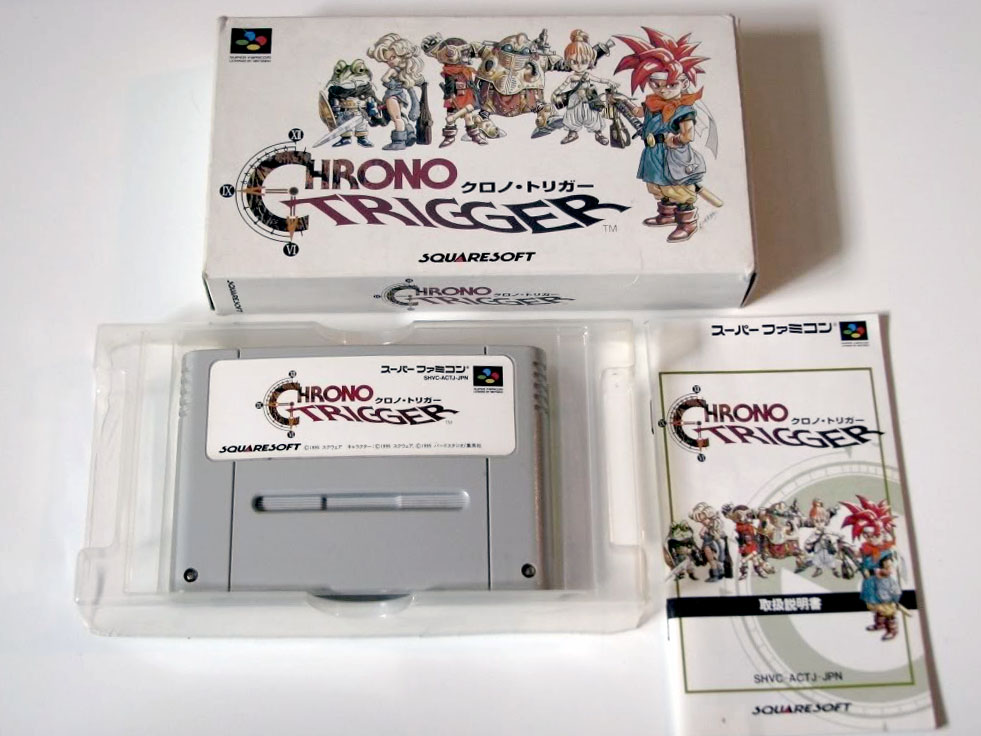
\includegraphics[width=0.5\textwidth]{gamecart}
 \caption{SNES Game Cartridge, 1995}
\end{figure}

As such, my method has been to focus on user-centered design to overcome the difficulties of migrating skills involved in one creative practice, video design, to a second practice – game design, or user-centered narratives. ScreenPerfect's initial layout and idea of operation was designed with a video artist – Hannah Epstein - who laid out an idea for how an interaction might work. The interaction was duly written, then released, refined, and redeveloped for a broader audience via the inclusion of editing tools, who then created games of their own. The hope is that each new version of the tool will generate a useful echo chamber, amplifying and iterating new ideas and tools even as it makes advanced technology easily accessible to content producers.

The toolset can then be released and left for artists to use and analyze, and can be expected to run 
privately on optimized systems similar to game cartridges from the 1990s (Figure 1.1). Rather than actual cartridges, these installation kits take the form of locked SD cards or USB sticks, which can be relied upon to hold their data in a reliable, mobile format. This means that artists will be able to install and display their own games independent of any central server, free of what the technician might decide is the context of the work. This should permit reliable installation of completed works even in remote contexts – a forest, for example, or a desert (Figure 1.2). This is distinct from other systems in that it is built using contemporary technologies, but also in that it is built with an eye to permanent, disconnected installations that rely on contained frameworks and simple, contemporary script languages, rather than on translations of preexisting software such as Java.

\begin{figure}[!ht]
\centering
  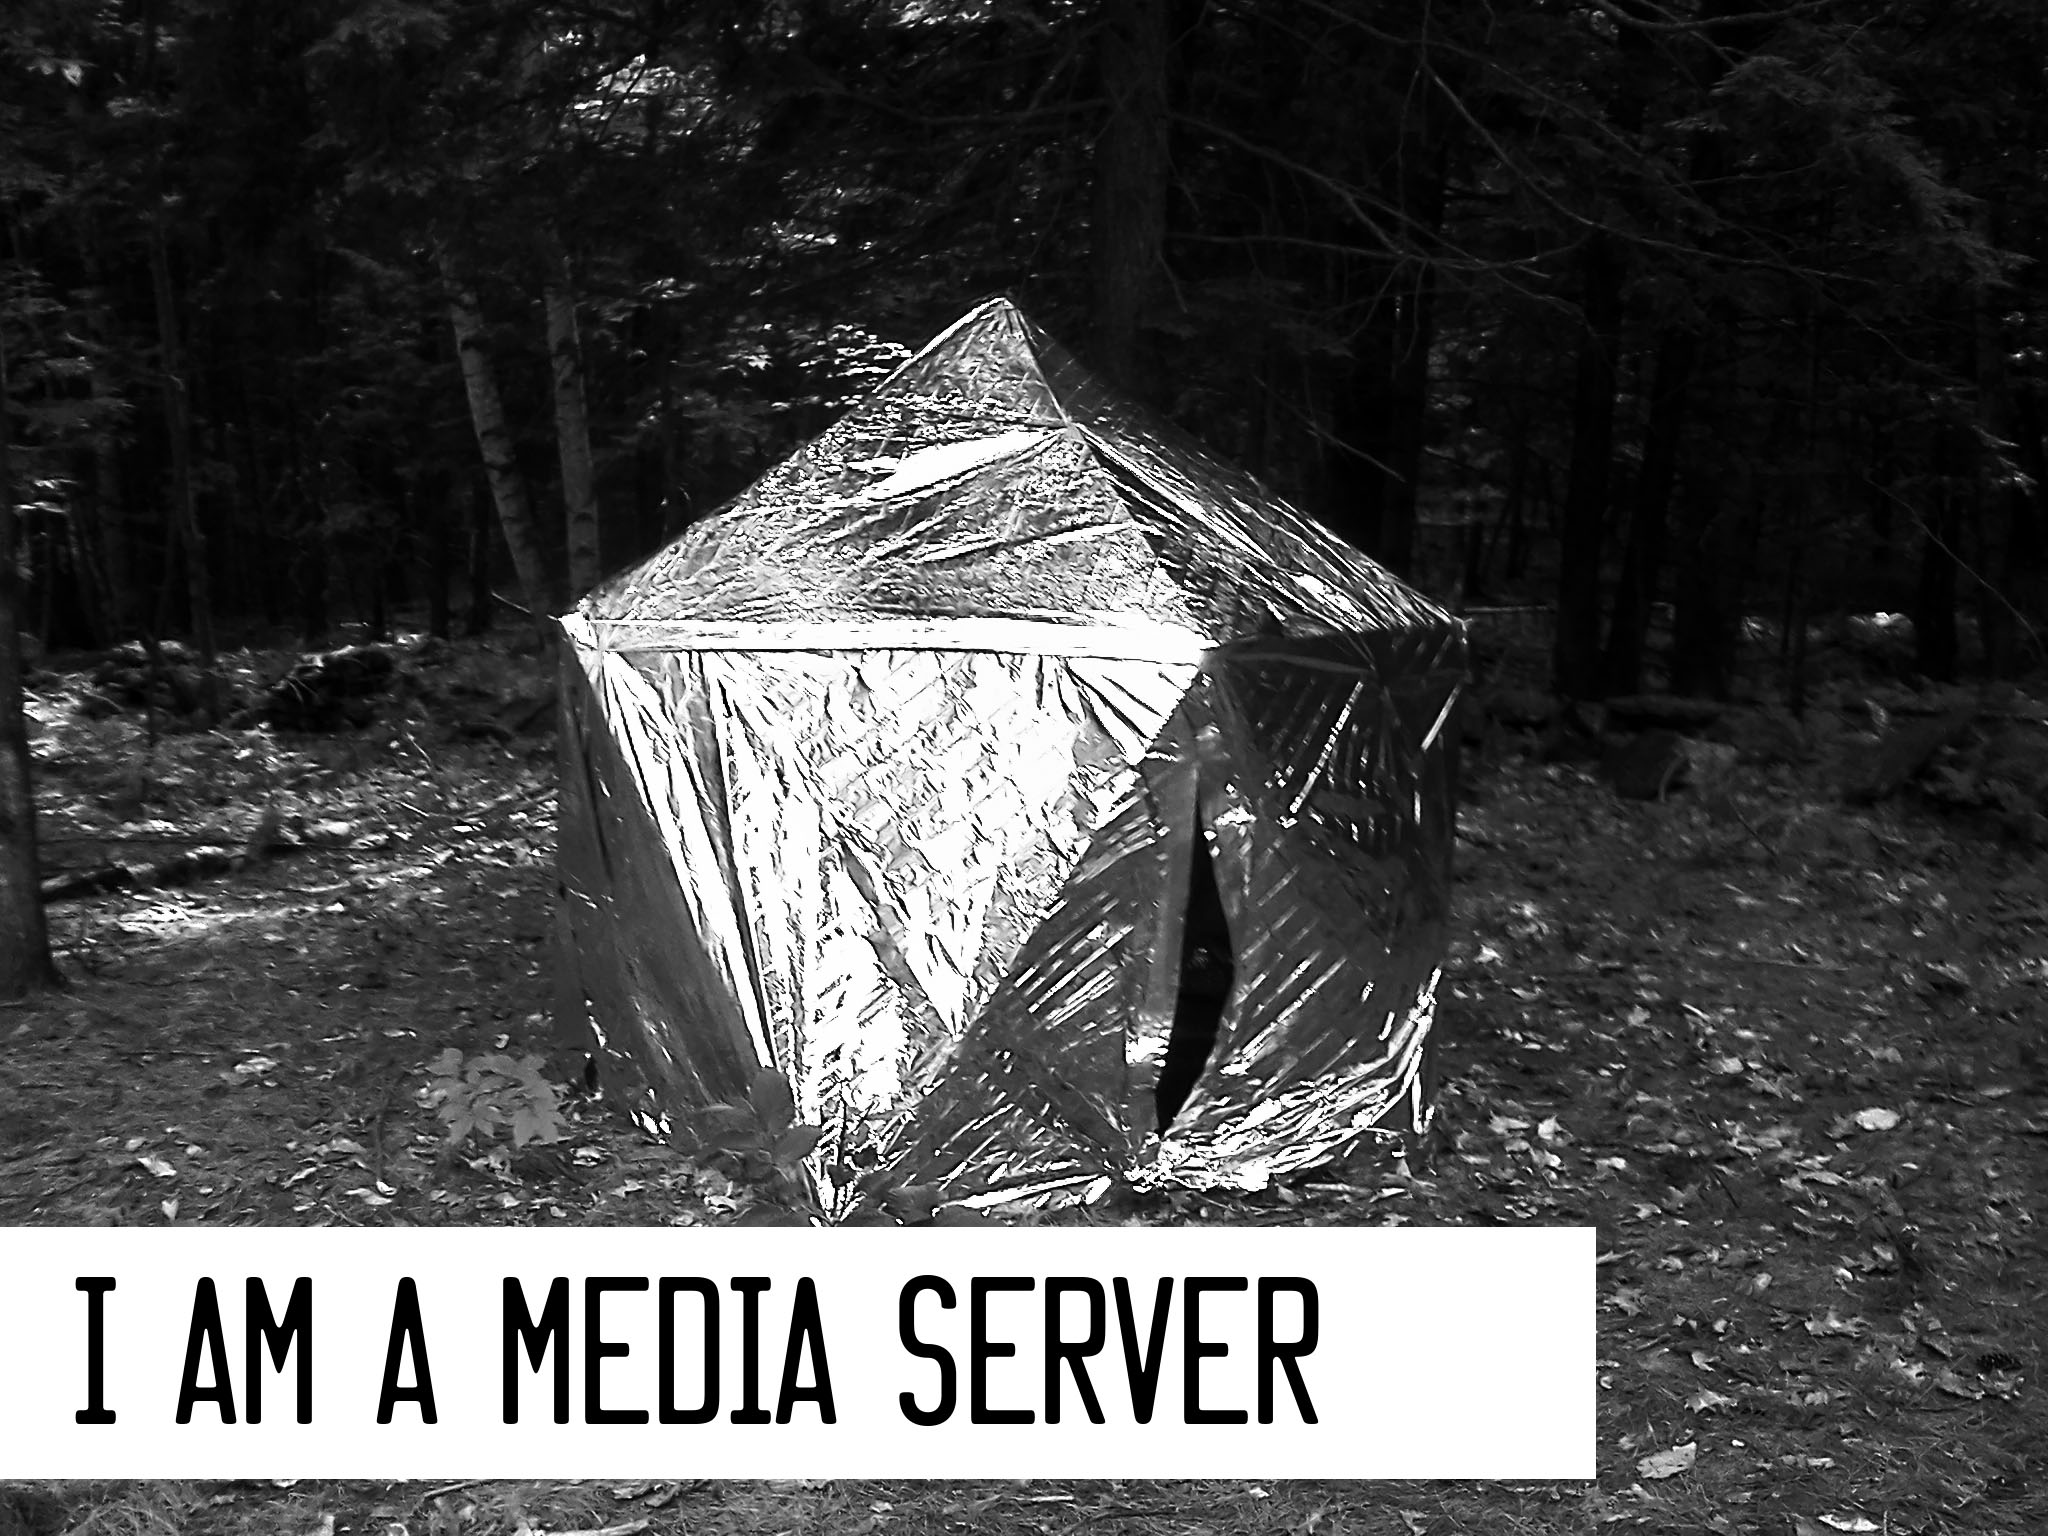
\includegraphics[width=0.5\textwidth]{Seizuredome2}
 \caption{Seizuredome, S. Kochavi, A. Shulz, 2013.\\ A tent with video installation.}
\end{figure}

\subsection{Code and Theory}
The initial software of this project was developed as a response to the lack of privacy and control of various shared media sources online. The project emerged from pairing with Hannah Epstein, who had an idea for a game featuring dual screens, but access to only commercial tools with limited potential for extensibility. Rather than producing exclusively an engine for a single production, it seemed reasonable to produce an entire editing environment, which would place the control of the final experience into the hands of the artist. This would in turn produce an engine that could be relied upon for public performance, but also an opportunity to easily make more than one game using this particular series of interactions. Video artists are already skilled technicians with a grasp of how to set a scene, so it seemed positive to extend their ability to easily piece together branched full-motion-video game works that would then display on the internet. 

Part of the motivation for this engine is that commercial engines tend to prioritise commercial distribution and mass experience, whereas artist installations tend to prioritise the direct experience of a specific work at a specific time. Although there are commercial FMV engines, they do not permit easy access to multi-screen synchronisation, and cannot be accessed offline. This meant that presenting the works developed using these systems meant agreeing to advertising, or to sign up for an account with the company, rather than being able to turn on an appliance and serve an art work.

The engine that drove psXXYborg worked well in practice, but the installation of multi-screen technology caused many issues. The technology, designed for multiple screens, required a great deal of technical support, as well as a very specific server that could be easily damaged - the mac mini - and keyboards, mice, as well as various power supplies. The total installation process for an early build of psXXYborg/screenPerfect has been detailed in Appendix A, "screenPerfect Installation Guide." The technical limitations of repeated equipment rental included tablets with permanent Google logins attached, inconsistent software environments, and web standards unevenly implemented across environments. Mobile computers in particular do not have any kind of consistent support for HTML5 video standards, the most common problem being that video will not play on load in some, but not other, HTML5 environments. This meant that in addition to custom software, consistent hardware was required for our installations.

The code of screenPerfect is written wholly in javascript via the Node.JS software framework. Node is a server environment intended to permit developers familiar with javascript to write code for both the browser client and the server without switching computer languages, as has been common practice until the release of Node. ScreenPerfect's design concept has proven popular, and in order to simplify the interface of the editing tools, it was forked by my industry partners, Bento Box|Miso – the business hosts of Dames Making Games - who are interested in the idea of new game engines as a use case for their language, Daimio \parencite{daimio}. Bento Box produced a clean variant of my editing interface in order to help me run a game jam to gather samples of what an FMV game might look like. In return, I gave them full permission to convert screenPerfect to their own language and to extend that engine into a new application called "iV." 

The critical theory that underlies my practice is a combination of French poststructuralism - Helene Cixous in particular - and contemporary writing on video games and the history of women in technology. By producing the software and content with the input of a local feminist collective, Dames Making Games (\url{http://www.dmg.to}), and as part of a wider feminist research network (SSHRC-funded Feminists in Games (\url{http://www.feministsingames.com})), I have grounded the work in a social justice driven practice which encourages women to take part in their own lives by learning how to interact with machines and communicate with the broader world.

\subsection{Game Design Research}
FMV games are an old format, relatively speaking. The FMV began almost as soon as chapter selection became available on the laser disc systems of the 1980s, with 1983's game "Dragon's Lair" by Rick Dyer and Don Bluth the first entry in what would become a strange sub-genre. FMV was successful through 1984, but quickly failed due to the expense of laser disc systems and the relative cost of game development, with the 1985 Halcyon system costing \$2000 - adjusted for inflation, \$4,347.88 in 2014 - and offering only two games. The most well-known FMVs outside of Dragon's Lair are Night Trap, released in 1992, and Phantasmagoria, from 1996 - Night Trap went on to become part of the congressional hearings of offensive video game material, along with Mortal Kombat, the first widely popular fighting game to allow people to rip out one another's spines. Phantasmagoria was better known as the first adult-oriented game released by Roberta Williams, famed for her involvement in Sierra's King's Quest point-and-click adventure game series \parencite{encyclopediavideogame}.

FMV and branched narrative games differ from cartridge-based action games in that they do not typically feature the same immediate feedback of a score going up and the instant player controls of a more typical 2D or 3D action game. Instead, players select what will happen next at key intervals. Older games are easy to display, so long as working hardware can be found, because they rely on consistent materiel for installation. New media interactive forms, particularly those on the internet, live in a more malleable format. They can change, or be taken down, at any time. The gameplay experience of a console game can be had even when disconnected from the internet – in fact, the Nintendo 3DS, a pocket console, outsold every other system on the market in 2013. It is speculated that its success is due largely to the fact that the 3DS is a portable system that does not connect to the broader internet unsupervised. This reliability is something that is rare to find in more complex computers: sometimes, as argued by Don Norman in "The Design of Everyday Things" \parencite{norman}, it is best to have a single thing do one thing really well. 

FMV games remain interesting enough to engage fans. They have been recreated using Youtube and preserved from laser discs and DVDs \parencite{laserdiscarcade}. Phantasmagoria can easily be found in complete playthrough on Youtube, where the annotation system makes recreating a point-and-click environment trivial (\url{https://www.youtube.com/watch?v=oAXC-MwfpHA}). Nonetheless, they were heavily systems-dependent and are tricky to develop, given the difficulties surrounding copyrighted video works and public distribution - how to transmit something that contains so many different pieces of video information?

Another example of portable electronic interaction is the smartphone. Mobile is a huge segment of the market, excellent for text messaging, talking, and playing games that separate an audience from each other. Initially this technology seems not so great for bringing people together in the same space. The privacy of the phone has been seen as undermining or distracting, but might be seen to have instead a lot of potential: people examine things one-on-one with their devices, and then will share them with their peers.

Smartphones are inherently private systems used in public places. This leads to a set of assumptions on behalf of interaction developers: an application is a private thing, paid for, and downloaded to a private space, whereas a web page is a public resource that can be viewed in private on a phone. A smartphone is also a single encapsulated controller, with all necessary inputs provided by its touch surface. For interactive artwork, this means that some assumptions can be made.

The first is that the audience of an interactive art piece is likely to be familiar with how to interact with a touchscreen, but also may be distracted. It cannot be assumed that they will download or pay for an application sight unseen for the sake of art, because that would constitute an expenditure of resources without reference, but they can be asked to go to a web page. People commonly use their phones in public, and therefore it seems reasonable to ask them for the minimal engagement of looking at something specific, this time art served only within the gallery. 

There are already games that aim to subvert this separation, and systems have been built to take advantage of the power of pocket computers. A notable effort is "Spaceteam," \parencite{spaceteam} a ‘Simon-Says' game for teams of up to four players. The application pairs to itself across phones by using a common network connection, and players in the same physical space cooperate to pilot a star ship. This allows players to make use of a device with which they are already comfortable to cooperate and share an experience.

This shared experience makes it possible to privately host a public space. screenPerfect, a web application served locally, takes advantage of an assumed set of smartphone users in galleries having access to the internet in their pockets. The internet is both bigger and smaller than the wider network – the internet that includes Google and other multi-national internet corporations. Rather than relying on the external resources of remote servers, screenPerfect provides a private wiFi point and what is called a "captive portal" to let players pair with one another and the server, control a large screen, and interact with a piece of video art in a localized area. This means that an artist can control the exhibition space for their work, design the experience of the work, and ensure that their audience will experience the work in a context that makes sense. It also ensures that technicians can access the underlying engine should something go wrong during the installation.

\subsection{Feminism, Cybernetics, and System Controls}
This work is related to various texts of feminist or woman-oriented critical theory: Haraway's "A Cyborg Manifesto," TIQQUN's "Preliminary Materials Towards A Theory of the Young-Girl." Haraway's "Cyborg Manifesto," from 1989, reads in relation to the world before the internet, where TIQQUN's commodification of women ten years later – from 1999, shortly before the first of a series of devastating economic crashes – more neatly quantifies the value of young woman as commodity \parencite{cixous}\parencite{tiqqun}. Cixous' work seems an interesting way to look through the construction of self that the internet provides to people who would like to package and produce an image of themselves. Where Haraway would rather be a cyborg than a goddess, and TIQQUN insists that young women|perfect stereotypes are the ultimate product of empire, Cixous insists on an individual self-determination and presentation, even when such seems impossible in a world where the tools for communication are totally controlled from a distance. Cixous insists on rebellion with a sense of play, and on this being the responsibility of the individual even when it seems impossible. 

All of these texts have complicated thoughts about embodiment, which I have chosen not to address, as I am more interested in embodiment via the idea of a piece of writing having a perceptible effect. Code has this ability. When you touch a screen, writing – interpreted or compiled – controls what happens next. In this context, the \textit{écriture féminine} can mean literal social breakdown, or a very physical change in the environment. Cixous' concept describes a space where women required to write, even using imperfect language or tools, least they be written out by the dominant voices that surround them. Her work, produced in the 1960s, describes a deeply embodied form of resistance to a language that describes what women want purely in context with what society wants for their bodies. The ideas are vividly expressed in relationship mainly to sexuality, but desire runs deeper than that: desire can include the desire for agency, for authority over oneself and one's life. Cixous states that to write is to write oneself into history, or into being \parencite{cixous}, while playing all the while with the idea of flight versus theft. Piracy, associated with copyright protections which have done nothing to limit distribution of video over the internet, has been characterized as theft - \textit{voler}, in French. Women who code, similarly, are designing works that must simultaneously be pragmatically functional, and may express totally different priorities than those implied by the authoritative structures present in the language.

In a practical sense, when one produces a work via a creative practice, that work expresses something of how one thinks. Cixous provides a ripping manifesto in \textit{Laugh of the Medusa}: those who are different should produce work that reflects and presents what they want to see in the world. This is a position of resistance through joy. 

This approach addresses woman as an alien construct to the more conventional world of technology, which has become associated with a masculinist performance. This is unnecessary for the pure structure of good rules and the development, through that, of good software. This construct is relatively recent, as Nathan Ensmenger discusses in his work on the systematic exclusion of women from programming as a trade \parencite{ensmenger}.
Although artists are central agents of production of the invisible yet tangible value of the culture industry, they are not always the prime beneficiaries of the financial system that backs, stores, and distributes the results of that capital. This is capital as both skill and capital as resource distribution: computers are expensive. 

In this instance, the artist is a specific person: video artists and cinematographers, who have a wide array of highly-trained skills that produce incredible images, which can then translate into FMV games. The software developer is both an administrator - a designer of forms, processes, and workflows - and a creative collaborator in their own right, as their code will dictate how the audience engages with video works that respond according to programming. A good engineer codes an experience that is engaging without being visible, a body of work that recedes into the background to better present video works in new contexts. Paired together, new works can be produced that take advantage of both sets of technical facility to enable new, different stories to be produced and displayed.

To test this idea, I have approached people to produce videogames with the screenPerfect software in the context of a voluntary game jam – a type of collaborative space where participants work with digital tools to generate new games in a limited window – and then the results are compiled for display into an arcade machine for presentation.

